\chapter{Simulation studies of semi-visible jets}
\label{chap:svj}

\epigraph{Of darkness visible so much be lent, as half to show, half veil, the deep intent.}{--- Alexander Pope}

\initial{A}ccess to the dark side of the universe is under a complex lock, seemingly unbreakable judging by the efforts of the past. A portal bridging the visible world to a realm of dark \acrshort{qcd}, however, may be discoverable at the \acrshort{lhc}. This chapter is dedicated to simulation studies in the context of a novel search for \glspl{svj}, characterised by hadronic final states and moderate missing transverse momentum.

% Can pull from Section 35 of my lab book, and all the talks I and other people from the team have given (Presentations and talks/ folder, also Other peoples/ subdirectory). Can also pull from AN for theory, translation of some theory stuff into experiment, and analysis strategy

% Could send a copy of the thesis to the SVJ team once I've got a complete first draft of this chapter. They would only need to look at theory section for SVJ, and this chapter. But I'd probably want to send the whole document since there are references to sections/formulae elsewhere in the thesis, and links would break, otherwise


%=========================================================


\section{Analysis summary}
\label{sec:svj_overview}

The analysis in search for \glspl{svj} is formed of a collaboration amongst the University of Bristol, University of Maryland, University of Rochester, Universit\"{a}t Z\"{u}rich, and the \acrfull{fnal}. The \schannel production mode with the full Run-2 dataset of \acrshort{cms} is the subject of the current analysis, at the time of writing. A dijet final state with moderate \ptmiss is expected. The transverse mass of the dijet system \mT---calculated with Eq.~\ref{eq:transverse_mass_massive}---is used as the search variable. Confirmed by the distributions in this chapter for simulated signal, a peak close to \mZprime can be captured. With the inclusion of the \ptmiss, the resolution of \mT is better than simply the dijet mass (\mjj) which would otherwise be used to recover the peak. The authors of Ref.~\citenum{Cohen:2017pzm}also demonstrate that sensitivity is stronger with \mT over \mjj. Novel techniques are utilised, such as the development of a boosted decision tree to tag \glspl{svj} and distinguish them from mismeasured \acrshort{qcd} \glspl{jet}. % Remove space between citenum and next word since it already introduces a space

While no public material is currently available, a PhD thesis from a former collaborator (who contributed to the \schannel analysis) can be found in Ref.~\citenum{GiorgiaRaucoThesis}. It is a slight variation of the \schannel analysis as of September 2019, with concessions made due to thesis submission timeline constraints. However, it can be used as a reference to demonstrate the direction taken in the main ongoing analysis.

My contribution to the main analysis is predominantly the development and understanding of signal simulation in \MGvATNLO~\cite{Alwall:2011madgraph} for both the \schannel and \tchannel aspects of the model. As such, the remainder of the chapter is focused on their discussion. The code developed by myself to perform the simulation is being used for the future analysis of the \tchannel mode as well as a low-mass boosted \PZprime search.


%=========================================================


\section{Signal simulation overview}
\label{sec:signal_sim}

In the main analysis, \PYTHIAEIGHT~\cite{pythia82} is employed to generate the \schannel signal as it can parametrise all the relevant aspects of the model in a simple manner with high signal efficiency. \MADGRAPH is the often-preferred generator as it can handle more complex models and decays. A higher degree of customisation and tuning of parameters is also possible. For the \schannel mode, modelling of the hard process should be equivalent between \PYTHIA and \MADGRAPH at \acrfull{lo}. In the former, the properties, interactions, and decays of the dark sector particles are implemented via the \texttt{Hidden Valley} module, available from \PYTHIA~8.226. Samples generated with \MADGRAPH are hadronised by \PYTHIA as part of the full simulation chain within \acrshort{cmssw}. \Gls{jet} matching and filter efficiencies may noticeably reduce the final number of events. The \tchannel model is possible to parametrise in \PYTHIA, but due to its complexity \MADGRAPH is favoured. Hadronisation, however, is still performed by \PYTHIA. In all cases, signal samples are generated at \acrshort{lo}.

All the details for \schannel signal generation with \PYTHIAEIGHT is given in Chpts.~\ref{sec:svj_signal_pythia} and \ref{sec:svj_showering_pythia}. This avenue was developed primarily by collaborators at \acrshort{fnal}. An equivalent implementation from myself where the hard scatter is modelled in \MGvATNLO, as both an alternative and cross-check to the \PYTHIA version, is documented in Chpt.~\ref{sec:svj_signal_madgraph}. A description of the \tchannel process is also present in the section. The parameters defining the shower are synchronised between myself and the \acrshort{fnal} colleagues. Comparisons between the \PYTHIA and \MADGRAPH implementations are discussed in Chpt.~\ref{sec:svj_schannel_comparisons}.

For all spectra, no additional object corrections or selections are performed. Reconstructed \glspl{jet} satisfy the tight identification criteria given in Tabs.~\ref{tab:htoinv_jet_id_def_2016}, \ref{tab:htoinv_jet_id_def_2017}, or \ref{tab:htoinv_jet_id_def_2017} depending on the data taking year. The missing transverse momentum \ptmiss contains the type-I correction as outlined in Chpt.~\ref{subsec:objects_analysis_energy_sums}. Similarly, the rest of the objects in the ntuples contain at least minimal quality assurances prior to any analysis-level selection.

The distributions that pepper the remainder of the chapter are generated with 2016 detector conditions and reconstruction. As the analysis began in 2017, the 2016 dataset was the only complete one intending to be used. Since it was the most mature and had been studied in depth by the Collaboration, the simulation should be representative of what could be observed in the data from that period. Selecting one year also ensures consistency across all of the plots even though they should not significantly change year-to-year.


%=========================================================


\section{Generation in \texorpdfstring{\PYTHIA}{Pythia}}
\label{sec:svj_signal_pythia}

The \texttt{Hidden Valley} module allows for simulating $\HepProcess{\Pquark\APquark \to \PZprime \to \Pqdark\Paqdark}$, where the $\PZprime$ acts as intended---a vector portal between the visible and dark sectors. Since a small percentage of them are expected to decay visibly, the branching ratio to the six \acrshort{sm} quarks is set to 0.003 for each flavour. The remaining fraction of 0.982 decay to $\Pqdark\Paqdark$, where $\Pqdark$ is a Hidden Valley particle charged only under that gauge group. The masses of the \PZprime and \Pqdark, and the narrow width of the \PZprime for resonant production can be given. Showering in the dark and visible sectors is then performed as in Chpt.~\ref{sec:svj_showering_pythia}. For both the complete event generation, and for hadronisation in the case of \MADGRAPH generation, \PYTHIA~8.230 is used.


%=========================================================


\section{Showering in \texorpdfstring{\PYTHIA}{Pythia}}
\label{sec:svj_showering_pythia}

Once the hard process has been simulated, showering of the dark and visible particles is performed. This can be separated into three separate steps. The \emph{parton shower} itself is where undecayed free quarks and gluons fragment and radiate due to their high energies. At \emph{hadronisation}, the showered partons coalesce into composite hadrons due to colour confinement. Finally, the \emph{underlying event} is the simulation of the previous two steps for any additional, softer collisions that occur between constituents of the incident particles, separate from the hard interaction. Often, the sum of all of these steps is just referred to as the \emph{parton shower} or \emph{hadronisation}.


%=========================================================


\subsection{Hadronisation of dark quarks}
\label{subsec:svj_dark_hadronisation}

Dark quarks hadronise into one of two species of dark meson (as the number of dark flavours $\Nf = \text{2}$) that correspond to particles from the \texttt{Hidden Valley} module: \Ppidark and \Prhodark, that are pseudoscalar and vector, respectively. Each possesses flavour-diagonal and off-diagonal variants. They are generated probabilistically with a ratio of 1:3. Dark hadrons are set to decay invisibly with a branching fraction \rinv. Remaining decay modes are to \acrshort{sm} quarks via a virtual \PZprime since it is the leptophobic portal between the dark and visible sectors. Decays of \Prhodark are democratic, i.e., with equal probability to accessible \acrshort{sm} quark-antiquark pairs.\footnote{Top quarks are excluded in all cases, since in the scan of model parameters where the greatest sensitivity is predicted, the dark mesons are always too light to decay on shell to a \ttbar pair.} Specifically, \Prhodark particles with $\mDark > \text{2}m_{\Pbottom}$ have a $\text{1}/\text{5}$ probability to decay to a \Pup, \Pdown, \Pcharm, \Pstrange, or \Pbottom. For $\text{2}m_{\Pcharm} < \mDark < \text{2}m_{\Pbottom}$, \Pbottom quarks are excluded and the branching ratio increases to $\text{1}/\text{4}$ for the remaining species. The \Pcharm quark is removed---and branching ratio modified---in the same manner for $\mDark < \text{2}m_{\Pcharm}$.

The decays of the \Ppidark mesons, however, are through a mass insertion. They couple to the longitudinal component of the \PZprime, assumed to arise from a leptophobic Higgs sector in an analogous manner to the electroweak bosons. Running quark masses are accounted for, as calculated in Ref.~\citenum{QCD_ESW}, since the decays are produced at the Higgs mass scale. Branching fractions to the \acrshort{sm} quarks are therefore based on the squares of the \emph{running} masses over the \emph{pole} masses. A graphical representation of the mass insertion decay is provided in Fig.~\ref{fig:svj_mass_insertion}.

% The mass insertion is briefly mentioned in the theory paper. Vector dark hadrons can decay promptly to SM quarks through the vector portal via the Z'. But scalar and pseudoscalar decays are suppressed by the mass insertion. Not sure how this affects the t-channel

\begin{figure}[htbp]
    \centering
    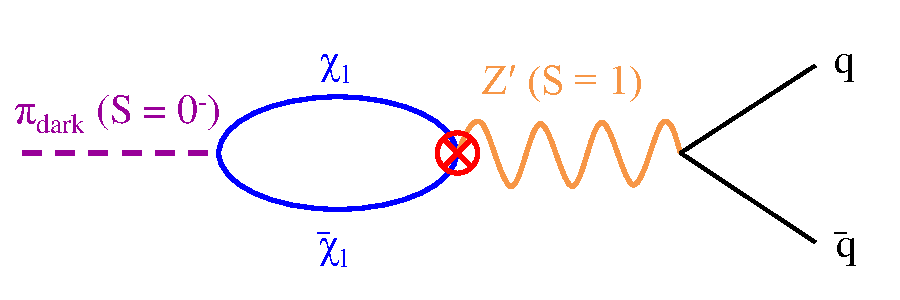
\includegraphics[width=0.5\textwidth]{figures/mass_insertion_diagram.pdf}
    \caption[A diagram of the mass insertion decay of \Ppidark mesons in the \schannel semi-visible jet model]{A diagram of the mass insertion decay of \Ppidark mesons in the \schannel \gls{svj} model.}
    \label{fig:svj_mass_insertion}
\end{figure}

The dark confinement scale \lamDark and running dark coupling \aDark are encoded based on the dark hadron mass as given below. \PYTHIA is now aware of the energy scales by which to hadronise and decay the dark sector particles. Final state dark radiation is also permitted, with a minimum \pt of $\text{1.1}\lamDark$ as imposed by \PYTHIA.


%=========================================================


\subsubsection{Simpler parametrisation of \texorpdfstring{\aDark}{alpha\_dark}}
\label{subsubsec:svj_effective_alpha_dark}

For simplicity, the values of \aDark used in the scan of parameter points are based on the value of \lamDark that maximises the dark hadron multiplicity in an event. The dependence is very small on \mZprime, and instead modelled as a function of \mDark by performing a fit. The value of \lamDark that leads to the largest number of dark hadrons (\lamDarkPeak) is
\begin{equation}
    \lamDarkPeak = 3.2 \mDark^{0.8}
    \label{eq:lambda_dark_peak_v_m_dark}
\end{equation}
which gives the parameter $\aDarkPeak = \aDark(\lamDarkPeak)$ calculated according to Eq.~\ref{eq:lambda_dark}. Variations on \aDark are calculated by scaling it by a factor 0.5 and 1.5, yielding $\aDarkLow = \text{0.5}\aDarkPeak$ and $\aDarkHigh = \text{1.5}\aDarkPeak$. For the purposes of emphasizing the effect of the choice of \aDark on the kinematics of the signal, an additional variation was introduced: $\aDarkVHigh = \text{2}\aDarkPeak$. The advantage of denoting the dark coupling strength with ``peak,'' ``low,'' and ``high,'' enables a more intuitive understanding of the parameter over a numerical value. Eq.~\ref{eq:lambda_dark_peak_v_m_dark} also means that \lamDark (and therefore \aDark) can be easily varied as a function of \mDark for each configuration of parameters in a scan of the model. Fig.~\ref{fig:svj_lamDark_vs_mDark} illustrates the evolution of \lamDark as a function of \mDark for each value of \aDark that is considered.

\begin{figure}[htbp]
    \centering
    \includegraphics[width=0.5\textwidth]{figures/lambda_dark_vs_mDark_with_vHigh.pdf}
    \caption[The dependence of the dark force scale \lamDark on the dark hadron mass \mDark for each value of \aDark used in the thesis]{The dependence of the dark force scale \lamDark on the dark hadron mass \mDark for each value of \aDark used in the thesis.}
    \label{fig:svj_lamDark_vs_mDark}
\end{figure}


%=========================================================


\subsection{Jet clustering}
\label{subsec:svj_pythia_jet_clustering}

The softer, visible radiation is simulated, and the clustering of \acrshort{sm} hadrons into \glspl{jet} happens in the hadroniser. The algorithm logic is known as ``sequential recombination,'' where particles are successively combined until certain criteria are met. In \PYTHIA, clustering stops above the merging scale known as the \texttt{qCut}, which is set to 125\GeV. For events generated in \MADGRAPH and interfaced with \PYTHIA for the parton shower, it is recommended that $\texttt{qCut} > 1.1 \texttt{xqcut}$. The \texttt{xqcut} denotes the merging scale in \MADGRAPH. Referring to the transverse momentum, the symbol $\kt$ is traditionally used in naming algorithms such as the \gls{antikt}. For consistency within this thesis, however, $\pt$ will be used.

For given particles $i$ and $j$, distance between them $d_{ij}$, and to the beam $d_{iB}$, are calculated as in Ref.~\citenum{schramm2016searching}:
\begin{equation}
    \begin{aligned}
d_{ij} &= \min(p_{\mathrm{T}i}^{2k}, \ p_{\mathrm{T}j}^{2k}) \frac{\Delta R_{ij}}{R^2},\\
d_{iB} &= p_{\mathrm{T}i}^{2k}
    \end{aligned}
    \label{eq:distances_kt_pythia}
\end{equation}
where, in the rapidity-azimuthal ($y$-$\phi$) plane, $R$ is a distance parameter related to the radius of the cone---defined as 1.0 to match the merging parameters used in \MADGRAPH. $\Delta R_{ij}$ is the separation between $i$ and $j$,\footnote{This is calculated with Eq.~\ref{eq:delta_r} where $\eta$ is replaced with $y$ from Eq.~\ref{eq:rapidity_def}.} and $k$ defines the algorithm choice: $k = -\text{1}$ in the \gls{antikt}, $k = \text{0}$ in the Cambridge-Aachen algorithm, and $k = \text{1}$ in the $\kt$ algorithm. The latter is chosen for the same reason as the cone radius size.

If $d_{ij} < d_{iB}$, the particles $i$ and $j$ are combined, replacing the individual constituents in the list of inputs. Otherwise, particle $i$ is designated as a jet and removed from list of inputs. For all combinations of particles remaining in the input list, the distances are recalculated until all objects possess a \pt above the merging scale. Once the algorithm has finished, all that remains are fully-clustered \glspl{jet}. Matching is performed between the clustered \glspl{jet} and original partons to avoid double counting. Events with insufficiently-matched \glspl{jet} are rejected. A minimum number of \glspl{jet} may also be specified and events with fewer than this are rejected. A larger $\rinv$ tends to reduce the merging and matching efficiencies since more energy is locked in the dark sector and fewer \glspl{jet} are clustered above the merging scale.

% Look in AN for more description regarding the dark hadrons, decays of dark mesons, etc. (https://gitlab.cern.ch/tdr/notes/AN-19-061/-/blob/master/sections/sigsamples.tex)


%=========================================================


\subsection{Filtering events}
\label{subsec:svj_pythia_filters}

Two filters are implemented in \PYTHIA that reject events with unrealistic decays: a $Z_2$ symmetry in the model requires invisibly decaying dark hadrons to produce the dark matter particles in pairs, and an invisibly decaying \PZprime must do so into a $\Pqdark\Paqdark$ pair. Coupled with the efficiency of the \gls{jet} matching and clustering algorithms---which only significantly affects events generated externally and decayed with \PYTHIA---there are multiple sources of inefficiency in the generation. Tuning the merging scale and matching parameters based on \rinv may yield in more effective generation. Aggregated over all sources, efficiency (in terms of the remaining event count) of the order of 15--20\,\% are expected for most \MADGRAPH samples.


%=========================================================


\section{Generation in \texorpdfstring{\MADGRAPH}{MadGraph}}
\label{sec:svj_signal_madgraph}

The \MADGRAPHFULL event generator is able to simulate the hard scatter for both the $s$- and \tchannel UV completions of the model, i.e., the decay of the \PZprime into $\Pqdark\Paqdark$ in the \schannel mode, and the exchange of the $\PBifund$ to transform $\Pquark\APquark$ into $\Pqdark\Paqdark$ in the \tchannel mode. Up to two additional \acrlong{sm} quarks or gluons may accompany the final state for either mode. The particles, couplings, and other parameters required to describe the models are defined using the \FEYNRULES package~\cite{Alloul:2013bka}. Of the four principal free parameters from Chpt.~\ref{subsec:theory_svj_free_params}, the mediator mass and \mqdark are defined at this stage.

The \schannel process is a modified version of the spin-1 ``DMsimp'' class of simplified dark matter models~\cite{Backovic:2015soa}. The \tchannel description is completely custom. Both were initially acquired by the analysis team from one of the authors of Ref.~\citenum{Cohen:2017pzm}at \url{https://github.com/smsharma/SemivisibleJets}. At the time, it contained only one set of mass points. For the work presented here, this has been greatly expanded allowing any combination of \PZprime, $\PBifund$, and \Pqdark masses and couplings. All signal samples produced with \MADGRAPH that feature in this thesis are done so with \url{https://github.com/eshwen/SemivisibleJets}. % Removing space between "Ref.~\citenum{Cohen:2017pzm}" and "at" otherwise it adds double space

In addition to the hard process, the full \acrshort{cmssw} simulation pipeline can also be executed. This enables hadronisation and decays of both the \acrshort{sm} and dark quarks in \PYTHIA (as detailed in Chpt.~\ref{sec:svj_showering_pythia}). The remaining free parameters of the model---\aDark and \rinv---are specified there. Subsequently, detector conditions and material interactions can be modelled in the 2016, 2017, and 2018 data taking periods of \acrshort{cms}. The parton distribution functions used in centrally-produced \acrshort{cms} simulation for each data taking period are also applied to these \gls{svj} samples for consistency.

Common to both the $s$- and \tchannel signal models generated for these studies, the couplings between the mediator and \acrshort{sm} quarks \gq---also the mediator and dark quarks \gqdark---are set to 1.0. Coupling strengths are furthermore independent of the dark and \acrshort{sm} quark flavours. The number of dark flavours and dark colours each have values of 2. Both affect the dark force scale as per Eq.~\ref{eq:lambda_dark}. Individually, former parameter allows for the production of two types of dark hadron, described in Chpt.~\ref{sec:svj_showering_pythia}, while the latter sets the dark colour composition of the dark gluon \Pgdark. 


%=========================================================


\subsection{\texorpdfstring{\MADGRAPH}{MadGraph} run settings}
\label{subsec:svj_mg_run_settings}

Somewhat decoupled from the parameters of the signal models themselves, there are many important, adjustable settings controlled by the run card that affect the behaviour of \MADGRAPH. The most notable of which is the parton/\gls{jet} merging scale, denoted as the \texttt{xqcut}. \MADGRAPH has difficulty simulating soft, collinear physics. To avoid this, a threshold may be placed on the \texttt{xqcut} to only generate sufficiently energetic events. Between two partons $i$ and $j$, the \kt is given as
\begin{equation}
    \kt^2 = 2 \min(p_{\mathrm{T}i}, \ p_{\mathrm{T}j}) [\cosh(\eta_i - \eta_j) - \cos(\phi_i - \phi_j)]
    \label{eq:svj_mg_kt}
\end{equation}
where $\eta$ and $\phi$ are the pseudorapidity and azimuthal angle, respectively. Complete definitions are presented in Chpt.~\ref{subsubsec:geometry}. Events with $\kt < \texttt{xqcut}$ are not simulated. In essence, the \texttt{xqcut} is a measure of the required separation between partons in the event. A value of 100\GeV is set in the analysis for consistency with Ref.~\citenum{Cohen:2017pzm}. This interpretation of a merging scale is similar, but not quite the same, as \PYTHIA's discussed in Chpt.~\ref{sec:svj_showering_pythia}.

The choice of parton distribution function also lives in the run card. As stated above, this changes to reflect the data taking period that is emulated. Preferences for particle separation, momentum and direction cuts, beam energy, and the \acrshort{qcd} renormalisation and factorisation scales are some of the additional settings that can be customised.


%=========================================================


\subsection{\texorpdfstring{\schannel}{s-channel}}
\label{subsec:svj_signal_madgraph_schannel}

In the description of the \schannel model, the leptophobic \PZprime is a spin-1 boson with vector couplings to the dark and \acrshort{sm} quarks. A width $\Gamma_{\PZprime} = \text{10}\GeV$ is specified; small enough to allow its resonant production. The dark quarks themselves are Dirac spinors with dark colour quantum numbers. Real and complex scalar dark quarks also exist in the files detailing the model, but are decoupled and not generated in this implementation. Consideration of these supplementary species of particle are beyond the scope of this thesis.

Cross sections for this process are calculated at \acrshort{nlo} as a function of \mZprime, assuming resonant production and a universal quark coupling. Events in simulation are weighted by the cross section multiplied by integrated luminosity of the full Run-2 dataset for an estimation of the production rate over this era of the \acrshort{lhc}. % Tracing back through the code used to calculate the cross sections, and what I think is the paper Nhan Tran was on for the dijet search, I think the cross section calculation comes from https://arxiv.org/abs/1306.2629, maybe more explicitly from slide 68 of https://indico.cern.ch/event/818454/contributions/3418046/attachments/1866479/3069375/CMS_PF_June20.pdf

It is important to understand the influence each free parameter of the model exerts on the kinematics of the final state. In which observables the variations of a given parameter manifest can aid in disentangling potential signal from background. The sensitivity, or lack thereof, of a parameter on the search variable also creates a sensible range for which to constrain the set of signal samples that must be generated. Signal models are given a label as SVJ\_\-$\expval{m_{\mathrm{mediator}}}$\_\-$\expval{\mDark}$\_\-$\expval{\rinv}$\_\-$\expval{\aDark}$. A benchmark point was chosen in the analysis with $\mZprime = \text{3000}\GeV$, $\mDark = \text{20}\GeV$, $\rinv = \text{0.3}$, and $\aDark = \text{peak}$, labelled as SVJ\_\-3000\_\-20\_\-0.3\_\-peak. The choice is motivated by Ref.~\citenum{Cohen:2015toa}and considerations of the other attributes of the signal provided in this chapter. Fig.~\ref{fig:svj_mg_benchmark_variations_schannel} shows the \mT in the case where a single free parameter is varied with respect to the benchmark point. A glimpse into the sensitivity of the parameter on the kinematics is evident.

\begin{figure}[htbp]
    \centering
    \begin{subfigure}[b]{0.48\textwidth}
        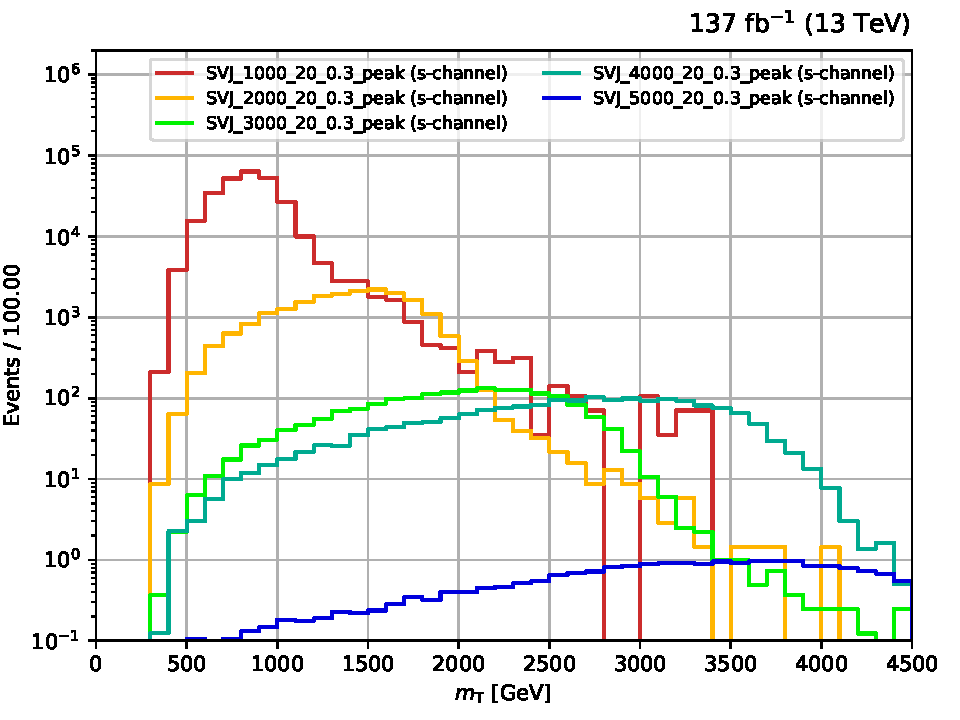
\includegraphics[width=\textwidth]{figures/s_channel_benchmark_variations/mZp.pdf}
        \caption{Varying \mZprime}
    \end{subfigure}
    \hfill
    \begin{subfigure}[b]{0.48\textwidth}
        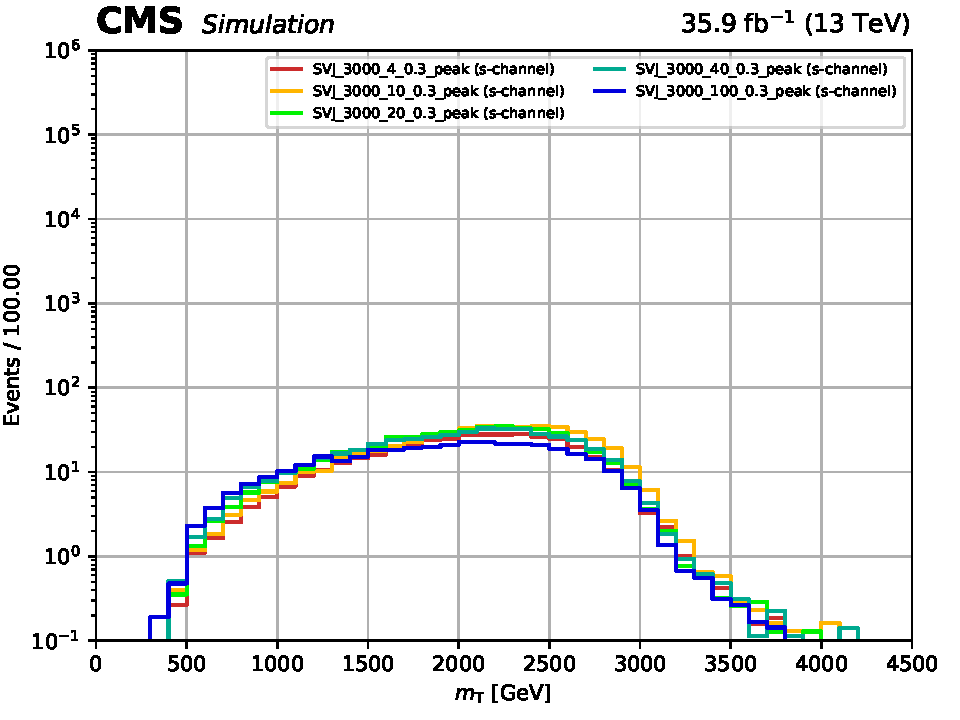
\includegraphics[width=\textwidth]{figures/s_channel_benchmark_variations/mD.pdf}
        \caption{Varying \mDark}
    \end{subfigure}

    \begin{subfigure}[b]{0.48\textwidth}
        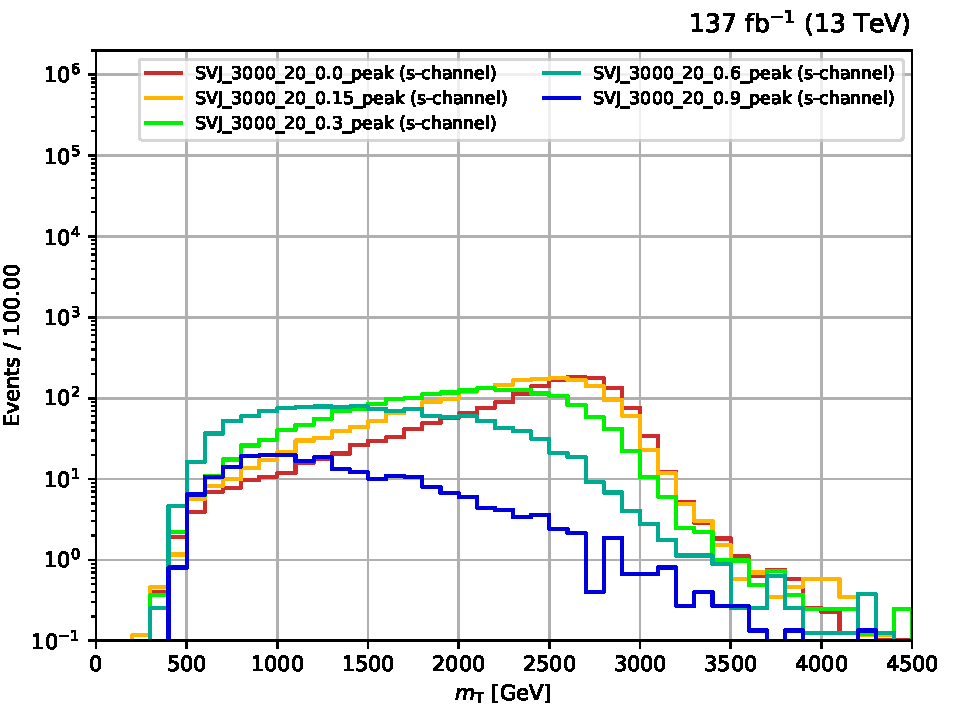
\includegraphics[width=\textwidth]{figures/s_channel_benchmark_variations/rinv.pdf}
        \caption{Varying \rinv}
    \end{subfigure}
    \hfill
    \begin{subfigure}[b]{0.48\textwidth}
        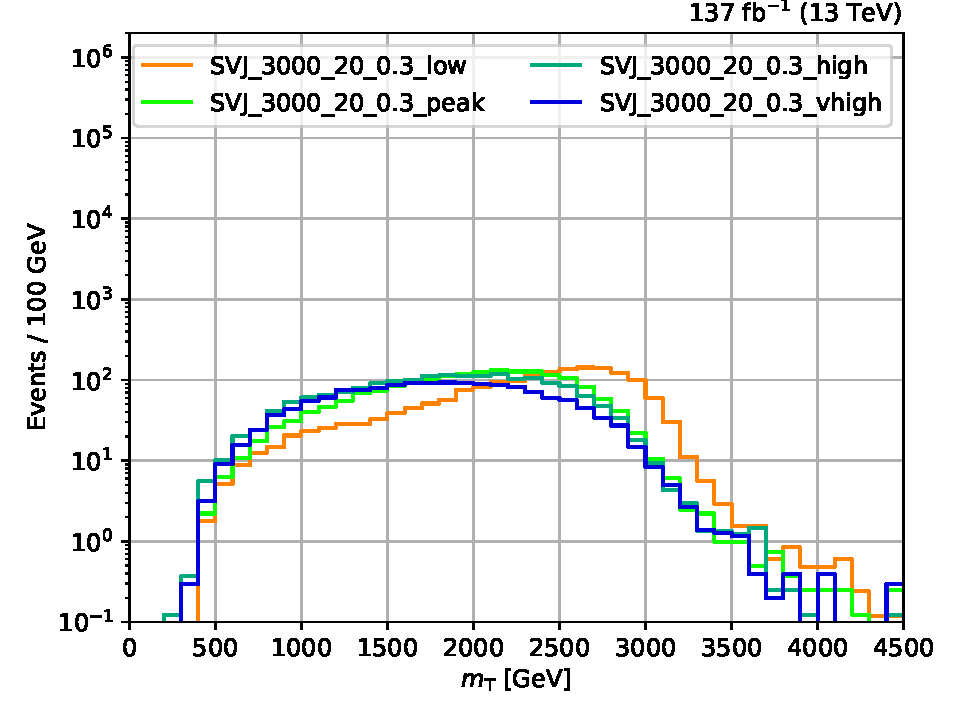
\includegraphics[width=\textwidth]{figures/s_channel_benchmark_variations/aD.pdf}
        \caption{Varying \aDark}
    \end{subfigure}
    \caption[Distributions of the transverse mass of the dijet system \mT for \schannel \gls{svj} samples emulating the 2016 data taking period. In each panel, one of the free parameters of the model is varied with respect to the benchmark point SVJ\_\-3000\_\-20\_\-0.3\_\-peak]{Distributions of the transverse mass of the dijet system \mT for \schannel \gls{svj} samples emulating the 2016 data taking period. In each panel, one of the free parameters of the model is varied with respect to the benchmark point SVJ\_\-3000\_\-20\_\-0.3\_\-peak (bright green line).}
    \label{fig:svj_mg_benchmark_variations_schannel}
\end{figure}

Perhaps expectedly, \mZprime appears to have the largest influence on the kinematics of the signal. Both the normalisation and shape of the distributions are significantly affected. A lower \mZprime recovers the peak near the mediator mass more effectively. Surprisingly, varying the dark hadron mass does little to the distribution. Though, the transverse mass is more sensitive to the clustered \glspl{jet} and \ptmiss as a whole rather than the shower constituents themselves. The momentum of the \glspl{jet} will also be highly correlated to \mZprime since \mDark is usually small in comparison, boosting the dark hadrons significantly. Varying \rinv shows an interesting trend. A smaller value reshapes the \mT distribution toward the \mZprime peak. Since the visible \glspl{jet} in the system are naturally resolved better than the \ptvecmiss, recovering \mZprime is an easier task. Similarly to \mDark, the choices of \aDark featured only have a small impact on the \mT spectrum. As with \rinv, a smaller value leans more toward the \mZprime peak. This can only happen to a point, however, because a model with an \aDark value too small refuses to shower in \PYTHIA.

For both \mDark and \aDark, checking many other observables leads to the same conclusion given above: the kinematics of the model do not appear particularly sensitive to changes in those parameters. This can be a positive consequence as it reduces the phase space required in the search for \glspl{svj} and permits optimisation of the analysis for \mZprime and \rinv.


%=========================================================


\subsection{\texorpdfstring{\tchannel}{t-channel}}
\label{subsec:svj_signal_madgraph_tchannel}

For the \tchannel model, several pseudoscalar bifundamentals $\PBifund$ couple to fermionic dark quarks. While only one flavour of mediator exists for \schannel process, numerous exist for \tchannel. Each flavour of $\PBifund$ couples to a given \acrshort{sm} quark flavour, and is charged under electromagnetism with a value matching that of its coupled quark. The cross sections for this process are calculated by \madgraph at \acrshort{lo}, varying most strongly as a function of \mBifund. A small dependence on \mqdark is observed, and naturally no effect from \aDark or \rinv since they only act at the hadronisation step.

The \tchannel aspect of the signal has not been studied in as great a detail as \schannel. It also exhibits less distinguishing kinematic characteristics, making it more difficult to determine the phase space and discriminating variables to separate it from the \acrlong{sm} background. Nevertheless, simple distributions with a range of parameter points are presented. These are intended to demonstrate how it would manifest in the \acrshort{lhc}, and how different the signature is from the \schannel model. Motivated by the sensitivities demonstrated by the theorists in Ref.~\citenum{Cohen:2017pzm}, the benchmark point SVJ\_\-2000\_\-20\_\-0.5\_\-peak is chosen. As with the \schannel UV completion, each free parameter is varied individually with respect to the benchmark point, the results of which for the \mT distribution are shown in Fig.~\ref{fig:svj_mg_benchmark_variations_tchannel}.

\begin{figure}[htbp]
    \centering
    \begin{subfigure}[b]{0.48\textwidth}
        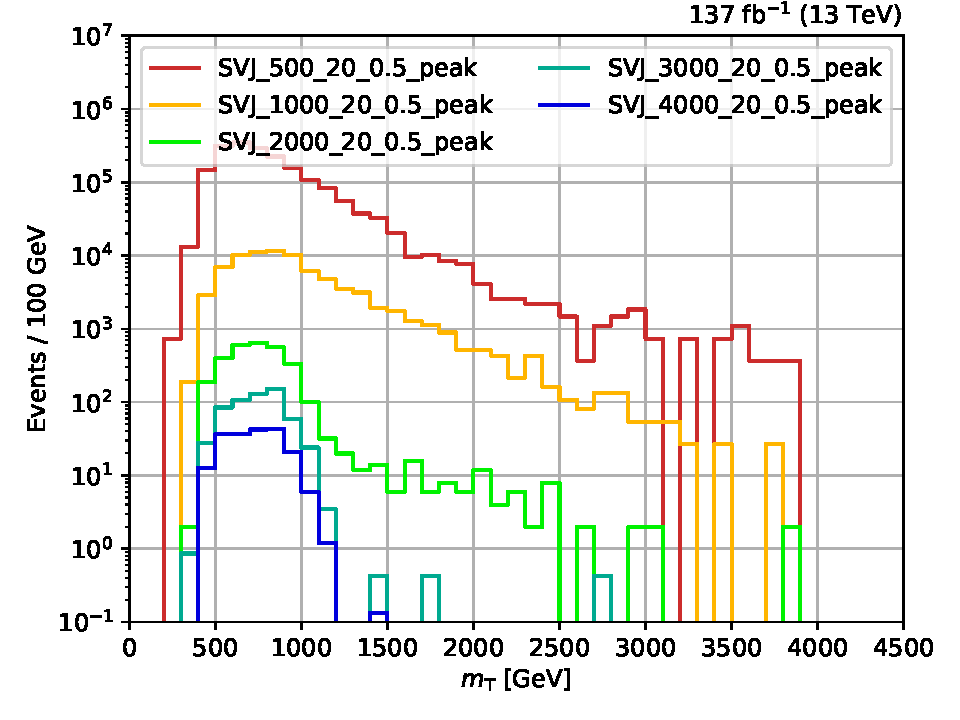
\includegraphics[width=\textwidth]{figures/t_channel_benchmark_variations/mPhi.pdf}
        \caption{Varying \mBifund}
    \end{subfigure}
    \hfill
    \begin{subfigure}[b]{0.48\textwidth}
        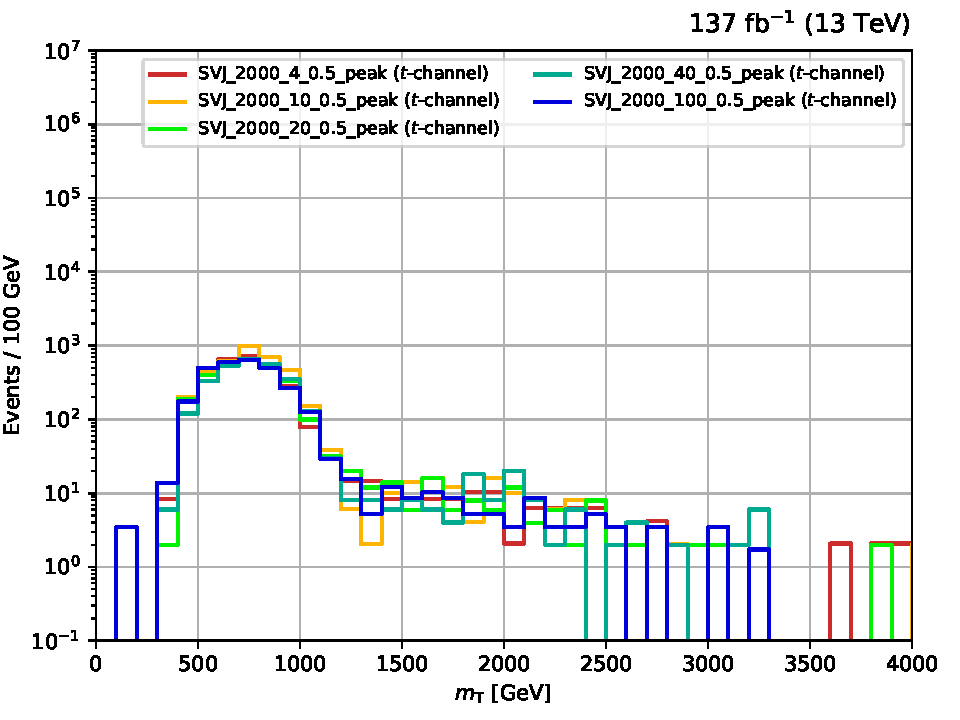
\includegraphics[width=\textwidth]{figures/t_channel_benchmark_variations/mD.pdf}
        \caption{Varying \mDark}
    \end{subfigure}

    \begin{subfigure}[b]{0.48\textwidth}
        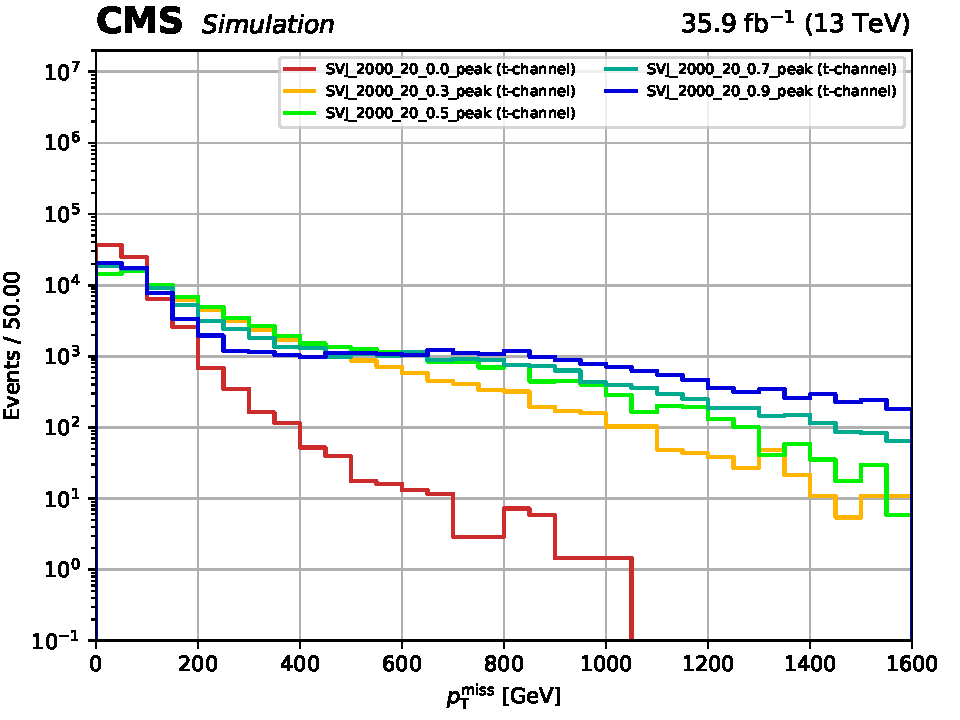
\includegraphics[width=\textwidth]{figures/t_channel_benchmark_variations/rinv.pdf}
        \caption{Varying \rinv}
    \end{subfigure}
    \hfill
    \begin{subfigure}[b]{0.48\textwidth}
        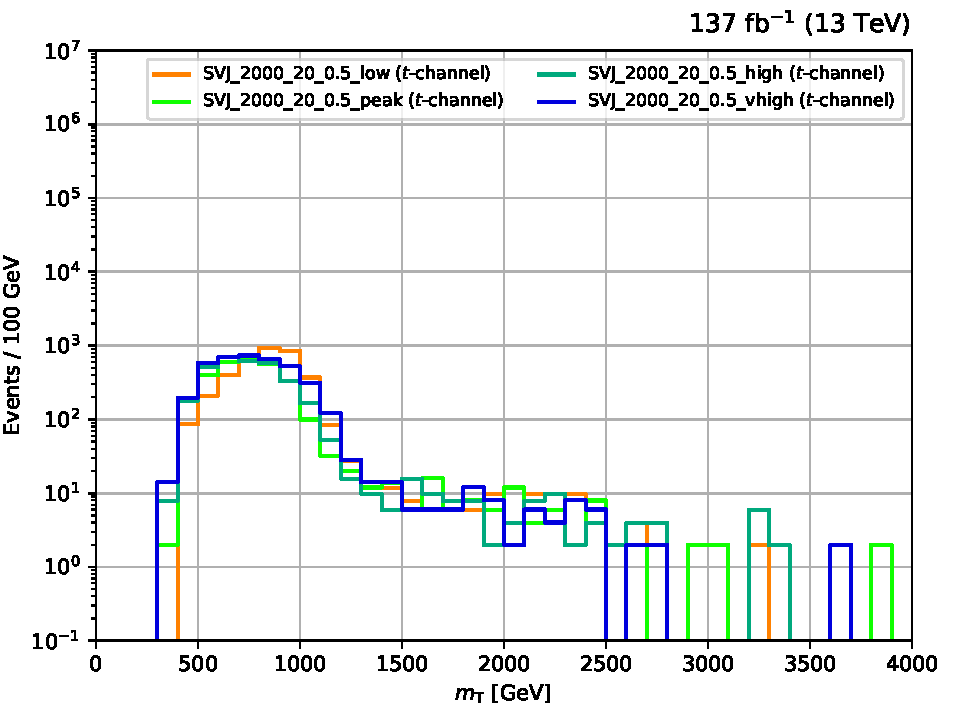
\includegraphics[width=\textwidth]{figures/t_channel_benchmark_variations/aD.pdf}
        \caption{Varying \aDark}
    \end{subfigure}
    \caption[Distributions of the transverse mass of the dijet system \mT for \schannel \gls{svj} samples emulating the 2016 data taking period. In each panel, one of the free parameters of the model is varied with respect to the benchmark point SVJ\_\-2000\_\-20\_\-0.5\_\-peak]{Distributions of the transverse mass of the dijet system \mT for \tchannel \gls{svj} samples emulating the 2016 data taking period. In each panel, one of the free parameters of the model is varied with respect to the benchmark point SVJ\_\-2000\_\-20\_\-0.5\_\-peak (bright green line).}
    \label{fig:svj_mg_benchmark_variations_tchannel}
\end{figure}

Analogously to the \schannel signal, the kinematics of the \tchannel aspect of the model are dominated by the mediator mass and invisible fraction. The transverse mass exhibits a peak, but consistently at 700--900\GeV, seemingly regardless of \mBifund. Shallower tails beyond the peak are seemingly observed for lower \mBifund, although the normalisation from the cross section may be partially responsible. Though this distribution is not as distinguishing as with \schannel since there is no resonance or equivalent kinematic edge, it is more discriminatory than other variables investigated such as \ptmiss or \HT. Lack of statistical precision dominates the curves at higher \mT for larger \mBifund. Accounting for this, however, and observing the general trend does reveal shapes comparable to smaller \mBifund. For low \mBifund, a reasonably large fraction of signal remains at high \mT. This is true in all panels of Fig.~\ref{fig:svj_mg_benchmark_variations_tchannel}, suggesting a cut could be placed on the observable to reject background if not used as the search variable.

\mDark and \aDark have little effect on the \mT. Within statistical fluctuations, the distributions for varying \mDark look identical. It is difficult to tell if \aDark has much effect on the kinematics overall, since the values used to vary the parameter are based on the shower of the \schannel signal. Reevaluation may be required in the \tchannel case. The \aDarkLow curve is peaked at slightly higher \mT than the others. With a lower threshold for dark hadronisation, a greater number of dark hadrons would likely be produced meaning a greater number that decay into visible hadrons. Since measuring the visible aspect of an event is more accurate than the \ptvecmiss, a more resolved peak would be observed.

The impact of \rinv on the \mT is similar to the \schannel signal insofar that the resolution of the bump is highly dependent on it. The peak near 1\TeV is recovered more effectively with a lower invisible fraction. Again, this is likely due to the enhanced resolution of \glspl{jet} over \ptvecmiss. The feature of identifying the peak at higher \mT with smaller \rinv may also be for the same reason.


%=========================================================


\section{\texorpdfstring{\PYTHIA}{Pythia}-\texorpdfstring{\MADGRAPH}{MadGraph} comparisons for \texorpdfstring{\schannel}{s-channel} signal}
\label{sec:svj_schannel_comparisons}

% Adding discretionary hyphen to split the long SVJ labels and avoid overfull hboxes

\PYTHIAEIGHT is described as a multipurpose generator, meaning it has the flexibility to simulate many kinds of processes from \acrshort{qcd} and electroweak \acrshort{sm}, \acrshort{susy}, technicolour, and leptoquarks. Its status as the de facto standard for the parton shower and hadronisation means interfacing between that step and the hard process is simple. The use of Sudakov form factors and resummation also yield realistic jet structure. However, it is difficult to simulate processes more complex than \acrshort{lo}, and support for generating new models must sometimes be specifically added to the program.

\MGvATNLO, on the other hand, is an automatic matrix element generator. It calculates the scattering matrix element for each subprocess for a given final state,\footnote{With these \glspl{svj} models, around 50 subprocesses exist for the \schannel mode, while approximately 820 exist for \tchannel.} with Feynman rules to generate each diagram within a subprocess. Integration is performed over the phase space for each subprocess to give the cross section. Generator- and phase space-level cuts are easy to implement, so that only signal in the phase space regions of interest are simulated. Systematic uncertainties from the generation step are also simple to extract in the situations they are important to an analysis. High order processes, such as \acrshort{nlo} and \acrshort{nnlo}, can be simulated. While extremely taxing computationally, it is a straightforward implementation on the user side.

To verify that both \PYTHIA and \MADGRAPH are suitable generators, 100,000 events were generated for a selection of parameter points with each program independently. Six models encompassing a sufficient range of \mZprime, \mDark, and \rinv were chosen: SVJ\_\-1000\_\-20\_\-0.3\_\-peak, SVJ\_\-3000\_\-20\_\-0.1\_peak, SVJ\_\-3000\_\-20\_\-0.5\_\-peak, SVJ\_\-3000\_\-20\_\-0.9\_\-peak, SVJ\_\-3000\_\-50\_\-0.3\_\-peak, and SVJ\_\-4000\_\-20\_\-0.3\_\-peak. For all the simulation steps after the initial generation (described in more detail in Chpt.~\ref{subsec:cms_mc}), identical implementations were used. This was to compare the differences due only to the generator. No analysis-level selections were applied either, for the same purpose.

Below are some of the important and insightful distributions for the \schannel production mode: \mT, the number of \glspl{jet} (with the large cone size equivalent to AK8 \glspl{jet} in the \gls{antikt}), the ratio of \ptmiss to \mT, and the minimum azimuthal angle between the \ptmiss and two leading \glspl{jet} $\dijetMindphi$. The ratio between the \MADGRAPH-generated and \PYTHIA-generated sample for a given model is also shown. For readability, plots are split into two sets comprising three models each. Fig.~\ref{fig:svj_mg_pythia_comparison_set1} showcases SVJ\_\-1000\_\-20\_\-0.3\_\-peak, SVJ\_\-3000\_\-20\_\-0.1\_\-peak, and SVJ\_\-3000\_\-20\_\-0.9\_\-peak, while Fig.~\ref{fig:svj_mg_pythia_comparison_set2} shows SVJ\_\-3000\_\-20\_\-0.5\_\-peak, SVJ\_\-3000\_\-50\_\-0.3\_\-peak, and SVJ\_\-4000\_\-20\_\-0.3\_\-peak.

\begin{figure}[htbp]
    \centering
    \begin{subfigure}[b]{0.48\textwidth}
        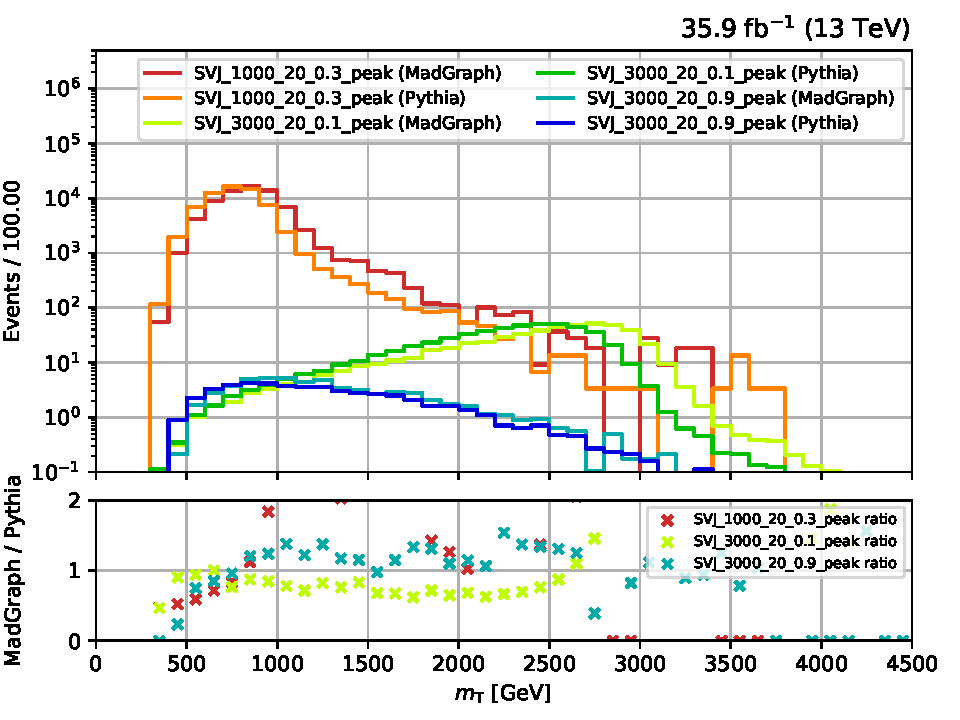
\includegraphics[width=\textwidth]{figures/madgraph_pythia_comparisons/plots/part1/dijet_mt.pdf}
        \caption{Transverse mass of the dijet system}
    \end{subfigure}
    \hfill
    \begin{subfigure}[b]{0.48\textwidth}
        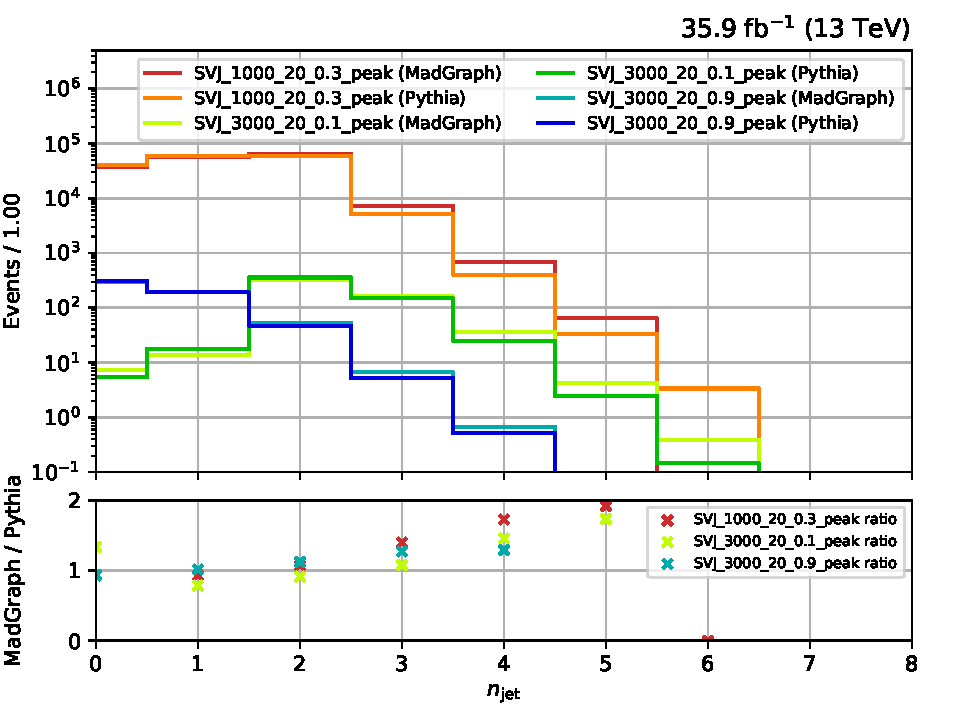
\includegraphics[width=\textwidth]{figures/madgraph_pythia_comparisons/plots/part1/njet.pdf}
        \caption{\njet}
    \end{subfigure}

    \begin{subfigure}[b]{0.48\textwidth}
        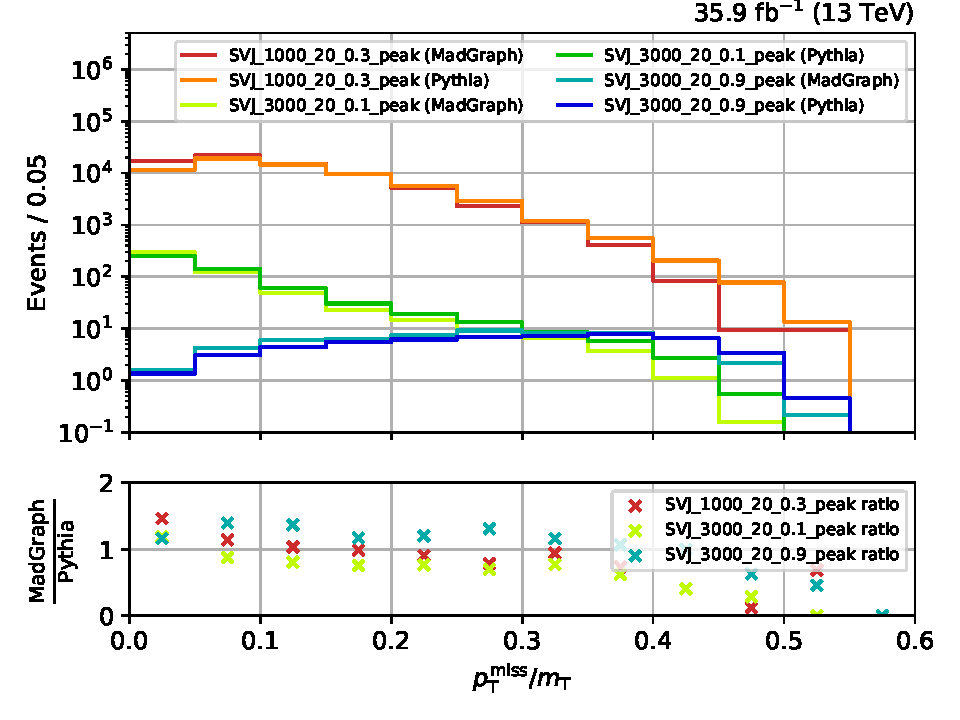
\includegraphics[width=\textwidth]{figures/madgraph_pythia_comparisons/plots/part1/met_over_mt.pdf}
        \caption{$\ptmiss/\mT$}
    \end{subfigure}
    \hfill
    \begin{subfigure}[b]{0.48\textwidth}
        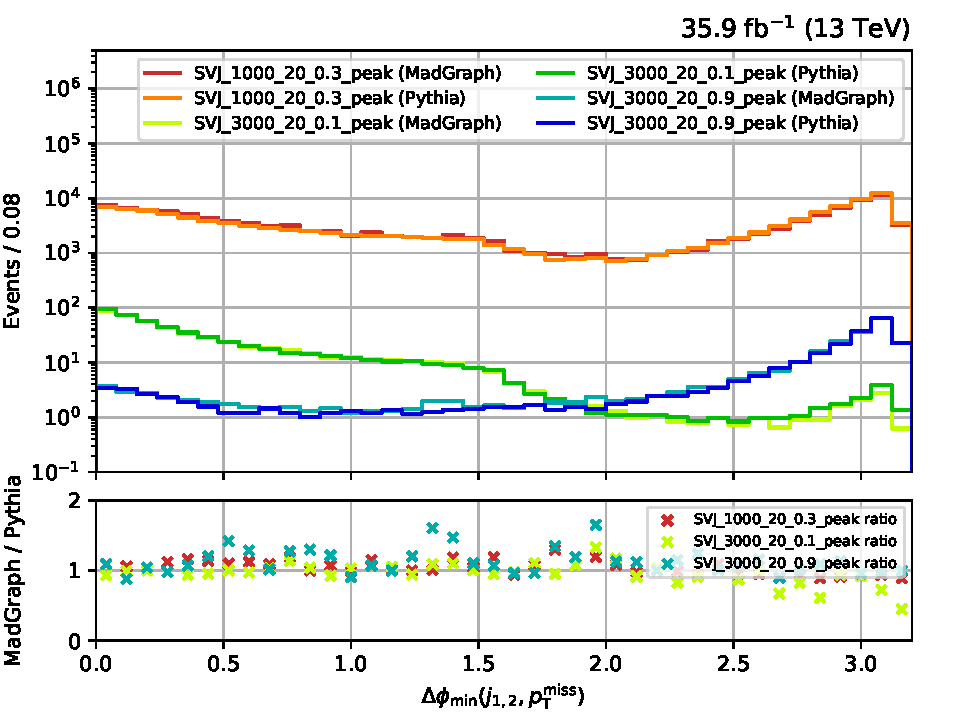
\includegraphics[width=\textwidth]{figures/madgraph_pythia_comparisons/plots/part1/min_dphi.pdf}
        \caption{\mindphi between \ptmiss and two leading \glspl{jet}}
    \end{subfigure}
    \caption[Distributions of several observables for the models SVJ\_\-1000\_\-20\_\-0.3\_\-peak, SVJ\_\-3000\_\-20\_\-0.1\_\-peak, and SVJ\_\-3000\_\-20\_\-0.9\_\-peak]{Distributions of several observables for the models SVJ\_\-1000\_\-20\_\-0.3\_\-peak, SVJ\_\-3000\_\-20\_\-0.1\_\-peak, and SVJ\_\-3000\_\-20\_\-0.9\_\-peak. Generation in \MGvATNLO is compared to \PYTHIAEIGHT, with the ratios between them for each model displayed in the respective subplot.}
    \label{fig:svj_mg_pythia_comparison_set1}
\end{figure}

\clearpage

\begin{figure}[htbp]
    \centering
    \begin{subfigure}[b]{0.48\textwidth}
        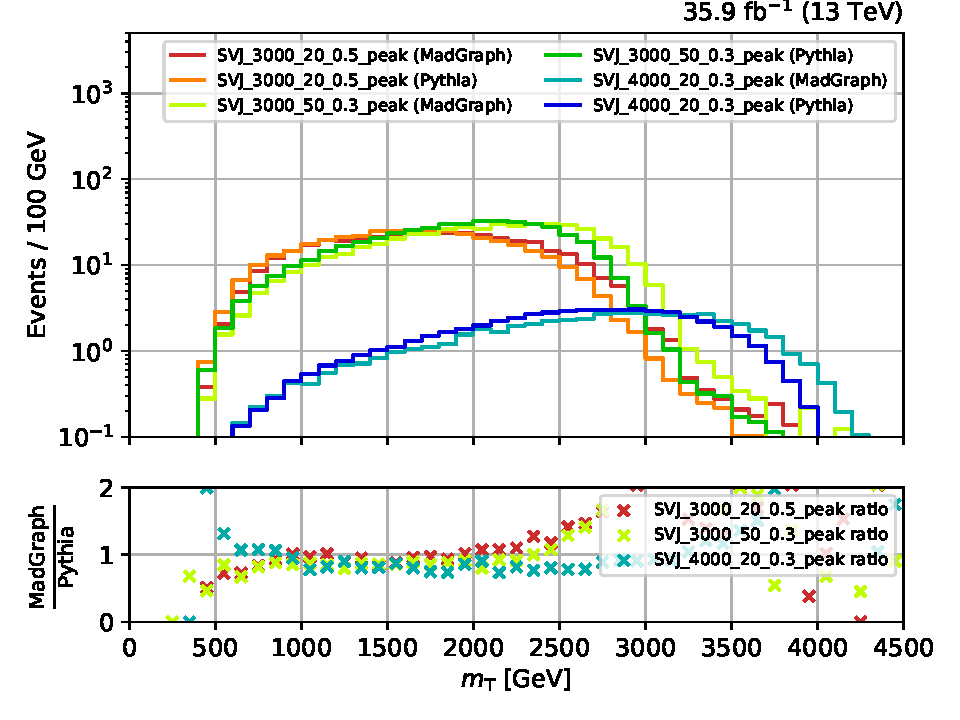
\includegraphics[width=\textwidth]{figures/madgraph_pythia_comparisons/plots/part2/dijet_mt.pdf}
        \caption{Transverse mass of the dijet system}
    \end{subfigure}
    \hfill
    \begin{subfigure}[b]{0.48\textwidth}
        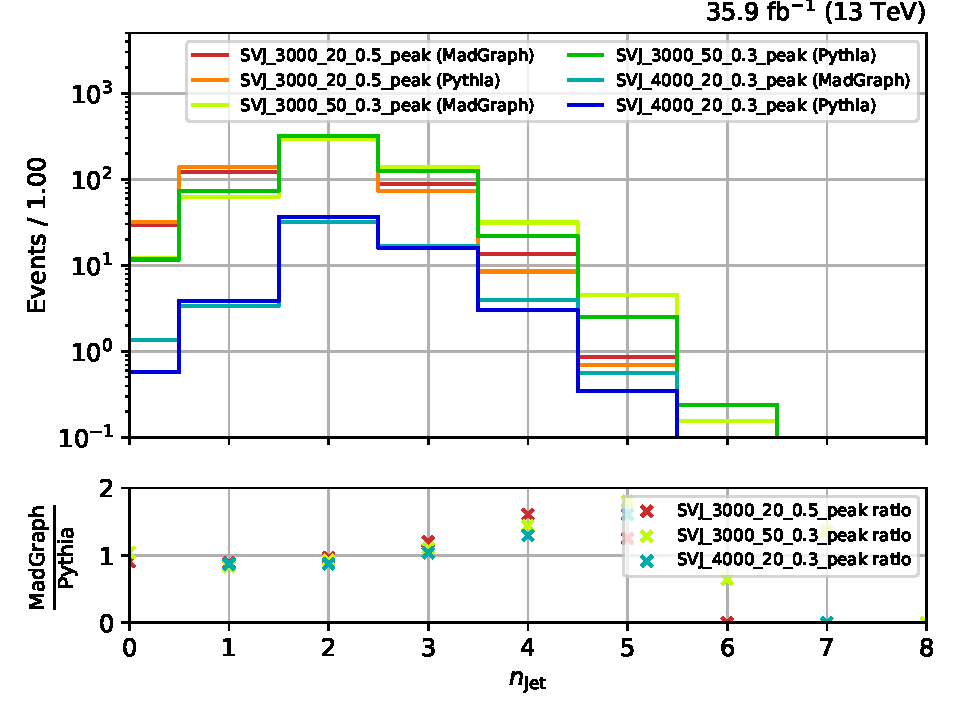
\includegraphics[width=\textwidth]{figures/madgraph_pythia_comparisons/plots/part2/njet.pdf}
        \caption{\njet}
    \end{subfigure}

    \begin{subfigure}[b]{0.48\textwidth}
        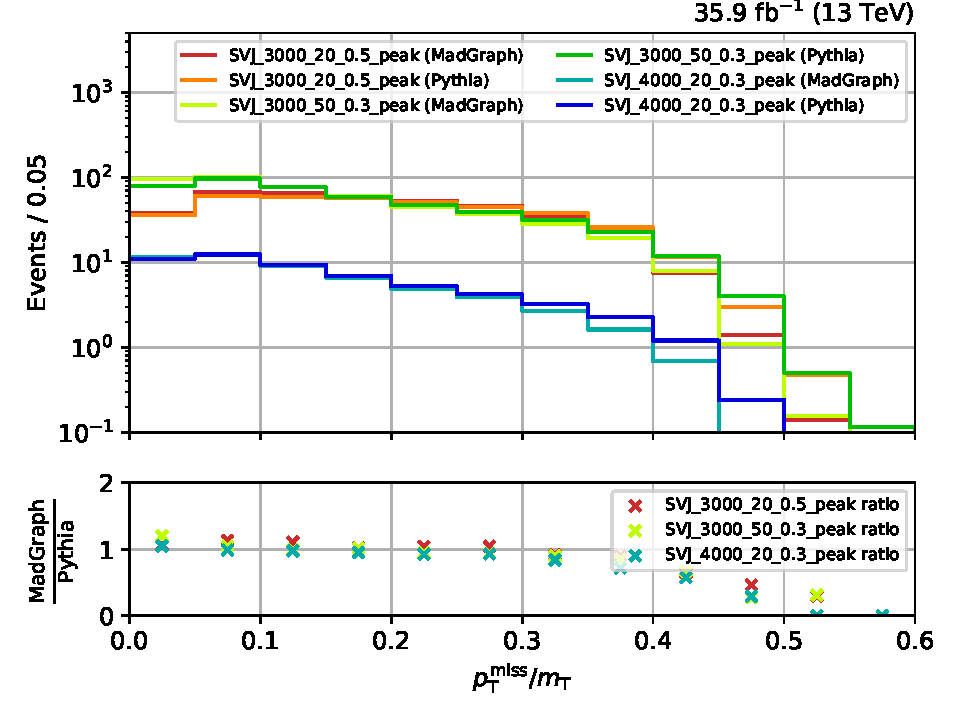
\includegraphics[width=\textwidth]{figures/madgraph_pythia_comparisons/plots/part2/met_over_mt.pdf}
        \caption{$\ptmiss/\mT$}
    \end{subfigure}
    \hfill
    \begin{subfigure}[b]{0.48\textwidth}
        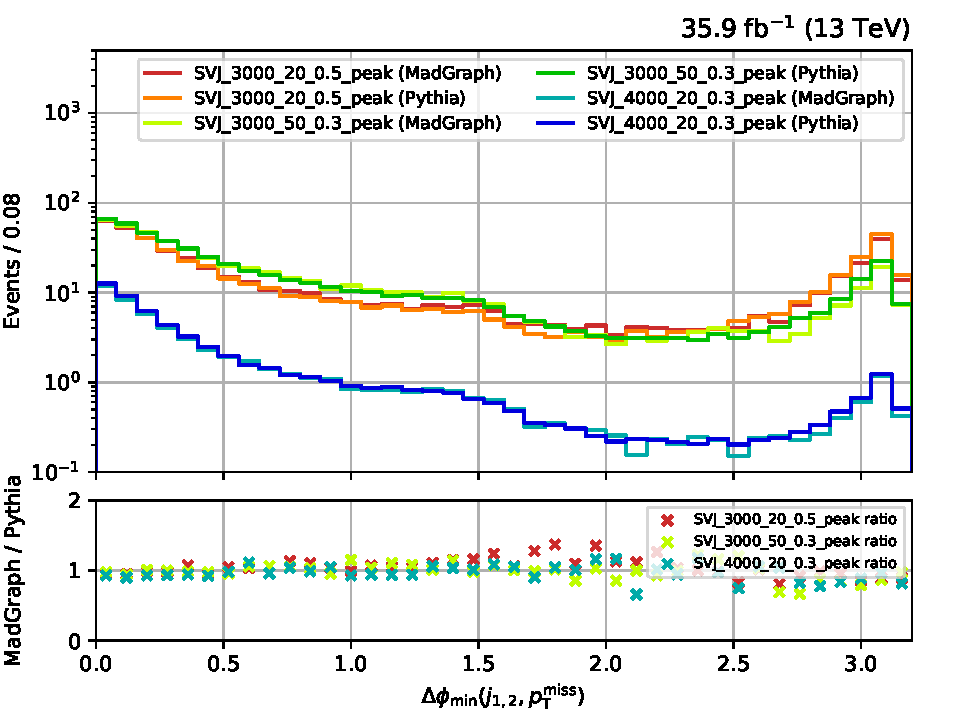
\includegraphics[width=\textwidth]{figures/madgraph_pythia_comparisons/plots/part2/min_dphi.pdf}
        \caption{\mindphi between \ptmiss and two leading \glspl{jet}}
    \end{subfigure}
    \caption[Distributions of several observables for the models SVJ\_\-3000\_\-20\_\-0.5\_\-peak, SVJ\_\-3000\_\-50\_\-0.3\_\-peak, and SVJ\_\-4000\_\-20\_\-0.3\_\-peak]{Distributions of several observables for the models SVJ\_\-3000\_\-20\_\-0.5\_\-peak, SVJ\_\-3000\_\-50\_\-0.3\_\-peak, and SVJ\_\-4000\_\-20\_\-0.3\_\-peak. Generation in \MGvATNLO is compared to \PYTHIAEIGHT, with the ratios between them for each model displayed in the respective subplot.}
    \label{fig:svj_mg_pythia_comparison_set2}
\end{figure}

In general, the distributions above---as well as the others investigated such as \ptmiss, \mht, and \gls{jet} \pt---show reasonable agreement between the two generators. In particular, position variables such as $\eta$ and $\phi$ of the \glspl{jet} and energy sums harmonise well. This is to be expected since those variables can be largely model-independent. A noticeable difference is in the \mT spectrum, where the shapes look similar but shifted to higher energies for the \MADGRAPH samples. This may be attributed to the \texttt{xqcut}, or differences in the \acrshort{qcd} scale. Tuning the \texttt{xqcut} in \MADGRAPH or \texttt{qCut} in \PYTHIA may be able to reduce the gap between them, especially if a relationship between the two merging scales can be derived for this model. For both generators, the peak close to the \PZprime mass can be recovered if the invisible fraction is small enough. This makes the transverse mass a more appealing search variable.

Both the \njet and $\ptmiss/\mT$ show trends in the \MADGRAPH/\PYTHIA ratio. A higher \gls{jet} multiplicity is seen in the \MADGRAPH samples, possibly due to the additional \glspl{jet} allowed in the matrix element calculation. For lower values of \rinv, a peak is seen at $\njet = \text{2}$, as expected given the theory. More \glspl{jet} may be generated from initial or final state radiation, or the dark shower prompting a large-width leading or subleading \gls{svj} causing one to be clustered as two. The larger invisible content of the high \rinv samples naturally shows a lower number of \glspl{jet}; fewer are likely to pass the \texttt{qCut} threshold since a larger momentum fraction of each \gls{svj} is invisible.

Larger values of \rinv in Fig.~\ref{fig:svj_mg_pythia_comparison_set1} manifest in an interesting \mindphi spectrum. A double peak structure is demonstrated in samples with lower values. In the case of dijet events, an imbalance in the invisible content of each \gls{svj} may cause the \ptmiss to be aligned with the one containing the largest invisible fraction. In other scenarios, one of the two \glspl{svj} may not be clustered if its invisible content is too large (i.e., if its visible content is too small). Then, in these single \gls{jet} events, the \ptmiss would appear to recoil from the only clustered jet. Higher values of \rinv would cause this to happen more frequently, mimicking a \acrshort{wimp} signature. Failing to cluster a \gls{svj} may also result in the muddied \mT distribution as the \ptvecmiss may not be resolved well enough.

For all of these comparisons, statistical limitation is an issue as it is only feasible to generate a rather limited sample size. Since those from \PYTHIA have, by design, a higher \gls{jet} matching and clustering efficiency, statistical power suffers partially for the \MADGRAPH samples. Higher efficiencies are usually achieved by samples with a lower \rinv---expected since \gls{jet} matching depends solely on the visible portion of the event.

In summary, an investigation has been performed into the generation and comprehension of the $s$ and $t$ production channels of \glspl{svj}. Progress has been made into understanding how simulated events would manifest in the detector, how variations of the important free parameters in the model affect the kinematics, and which variables would be sensitive in a search for them. The mediator mass influences the model's observable characteristics the most, affecting both the shapes of distributions and cross section significantly. Variables such as the transverse mass of the dijet system are able to emphasize the peak at the mediator mass in the \schannel mode, and to a lesser degree in the \tchannel mechanism. Effective discrimination between signal and the dominant backgrounds is expected. Comparisons between the \MGvATNLO and \PYTHIAEIGHT event generators were also conducted for several combinations of parameters in the \schannel aspect of the model. In most cases, reasonable agreement was found, with the major differences appearing to stem from the modelling of \glspl{jet}. Either would be suitable for use in the main analysis.

% For njet, typically see 2 jets as expected. Sometimes, the shower of one dark quark can spread large enough to be clustered as two jets. Then there's ISR and FSR. 2D plots of dphi(j1/2/3, MET) vs njet or something might be interesting to see where the MET is aligned 

% Generating 100,000 events. Obviously fewer end up in the plots from jet matching and filter efficiency
